\chapter{Indoor closures}
The interior of the terminal building has been designed so that users are able feel they are in an open space without vertical impediments, so the number of indoor closures is the minimum possible. The indoor closures are those spaces in which different activities are performed. The toilets are a clear example of this kind of areas, as well as those areas used by the airport staff.

	\section{Hallways}
For these spaces, an enclosure based on prefabricated partitions formed by plasterboards and isolating materials. The main advantages are the ease and speed of construction, it is economical, easy to maintain and has good thermal and acoustic insulating properties. In the hallways of the terminal building, good acoustic insulation is the most interesting factor to take into account, to separate the different areas dedicated to different activities and, in addition, a good fire resistance so that in case of having fire, it will be confined between partitions.
		
The partition supplier company is \textit{PLADUR\textregistered{}}, concretely it will be used the models \textit{PLADUR\textregistered{} F} and \textit{PLADUR\textregistered{} FONIC}. The first one is in accordance with the norm EN-520 and is formed by a plaster soul and glass fibre, which contributes to a better fire resistance. On the other hand, the second one is in accordance also with EN-520 and is formed by natural plaster soul recovered on its two faces by cellulose sheets specially treated so as to improve its acoustic insulation properties.

	\section{Offices}
These spaces do not have to be always placed in the same manner, it can present several distribution changes throughout its useful life, so it would be advisable to use a mobile or removable enclosure for an easy adaptation of the area according to the requirements of the moment.

The supplier company for these elements will be \textit{PROTECNICS GLOBAL}, concretely the model \textit{BUSINESS COMBI}, an elegant solution created to meet the needs of functionality and space (see Figure \ref{offices}). This model provides a high degree of personalization and a wide variety of solutions. It consists of a 100mm thick structure formed by extruded aluminium hidden profiles. On this structure, a double board of agglomerated wood of 19mm thickness covered in melamine will be placed, edged on its seen sides with 1mm of PVC and rock wool of 40mm thickness between panels. the panels will be anchored to the structure by means of an aluminium fixing system with a 2 mm thick neoprene seal. The glazed areas are provided with aluminium frames with rubber profile to seal perimeter, either the option of a single glass or double glass.

\begin{figure}[H]
	\centering
	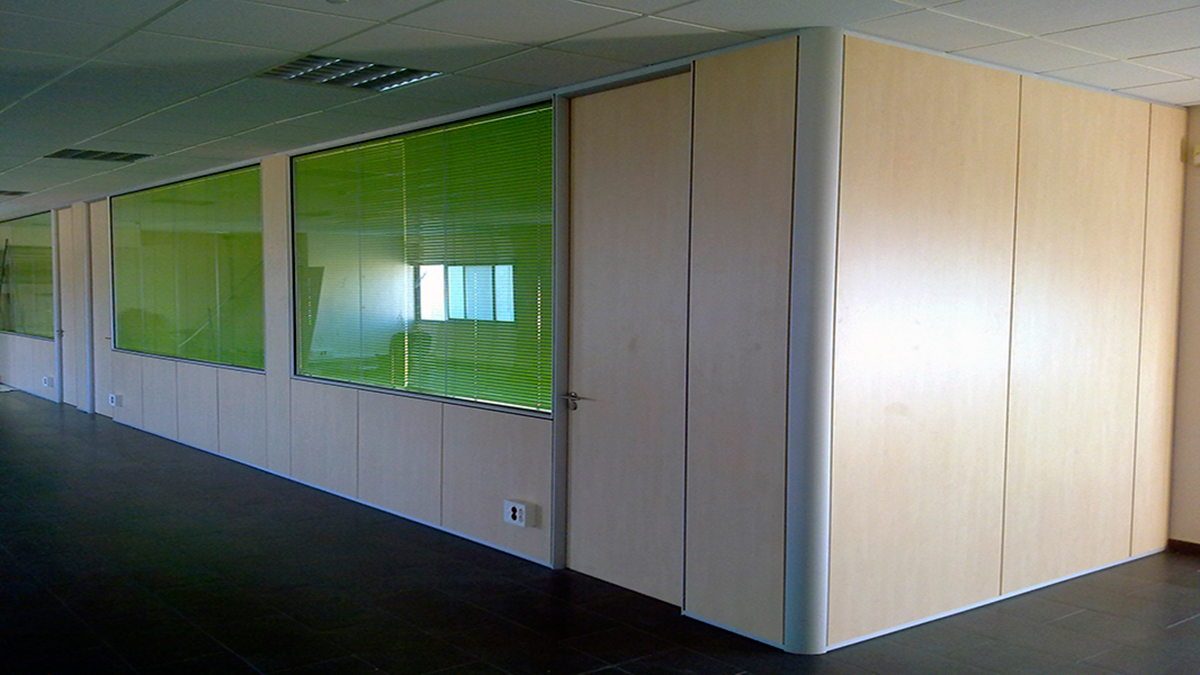
\includegraphics[clip, trim=0cm 0cm 0cm 0cm, width=0.8\textwidth]{./images/indoorclosures/offices}
	\caption{Terminal building offices provided by \textit{PROTECNICS GLOBAL}.}
	\label{offices}
\end{figure}


	\section{Passport controls}
Passport control facilities have to ensure the safety of the workers and users. For this reason, it will be used armoured materials. 

The solution adopted is to use armoured glass from the supplier company \textit{VITROMART\textregistered{}}, concretely the model \textit{Blindex\textregistered{}}. This model consists of sandwiching two sheets of glass and one polyvinyl butyrate (PVB) film, joining both parts by the simultaneous action of controlled heat and pressure, achieving an optimal optical quality sheet (see Figure \ref{passport}). It also offers a high range of protection against impact and penetration to it. At the same time it acts as an excellent barrier against sound.

\begin{figure}[H]
	\centering
	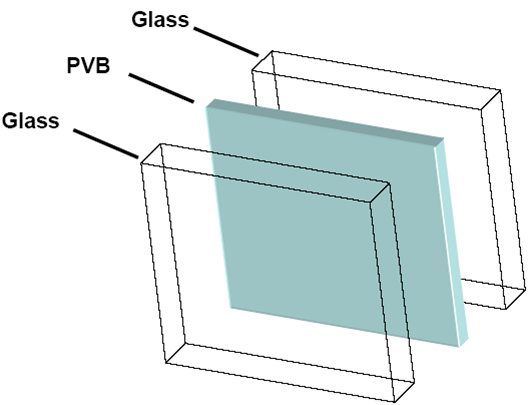
\includegraphics[clip, trim=0cm 0cm 0cm 0cm, width=0.6\textwidth]{./images/indoorclosures/passport}
	\caption{\textit{Blindex\textregistered{}} glass structure used for passport controls.}
		\label{passport}
	\end{figure}

	\section{Toilets}
For hygienic and odor reasons, it is necessary to separate the toilets from the common spaces and, in addition, it is required acoustic insulation. The enclosure must allow to support the necessary facilities to fulfil the function of toilet.

The best solution for these spaces is to use opaque and fixed enclosures, since in this case they are non variable elements, they will always be located in the same position. The most optimal solution for closing the toilets are in situ enclosures made with ceramic hollow blocks (see Figure \ref{block}). In this way, rows of blocks will be joined with cement mortar and a final coating based on tiles will be used (see Figure \ref{tiles}). These blocks will not have any structural requirement.

The company supplier of the blocks is \textit{CERAMICAS ARCIS} and the one supplying the tiles is \textit{ONDACER  S.L}.

\begin{figure}[H]
	\centering
	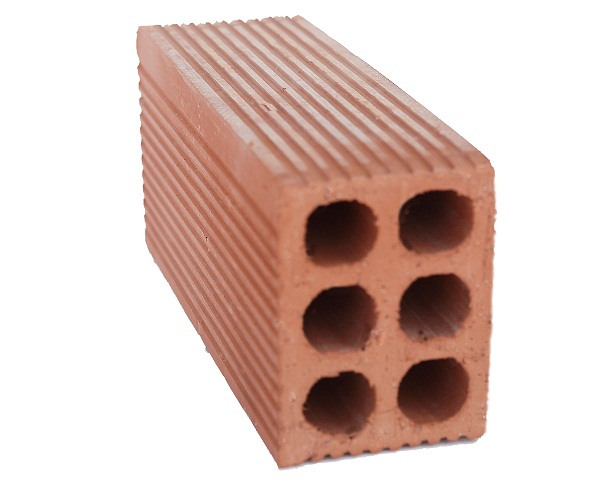
\includegraphics[clip, trim=0cm 0cm 0cm 0cm, width=0.4\textwidth]{./images/indoorclosures/block}
	\caption{\textit{CERAMICAS ARCIS} ceramic blocks used for the toilets.}
	\label{block}
\end{figure}

\begin{figure}[H]
	\centering
	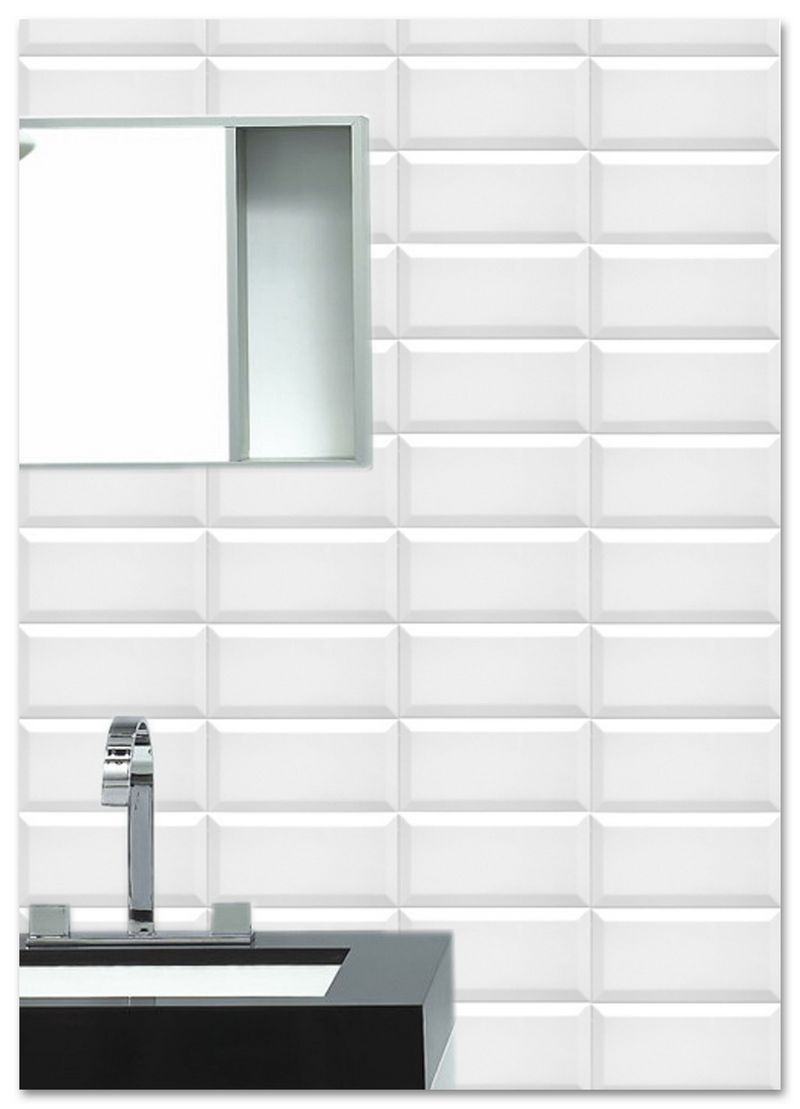
\includegraphics[clip, trim=0cm 0cm 0cm 0cm, width=0.3\textwidth]{./images/indoorclosures/tiles}
	\caption{\textit{ONDACER  S.L} tiles used for covering the ceramic blocks used for the toilets.}
	\label{tiles}
\end{figure}

	\section{Elevators}
Elevators are those elements allowing a vertical movement inside the terminal building. They must be able to charge a lot of people during the day, as well as all the luggage they take with them. In order to avoid claustrophobic attacks, the elevators have to be well illuminated and have to transmit a safety impression.

The solution adopted for the elevators is the \textit{SCHINDLER 5500} from the company \textit{SCHINDLER} (see Figure \ref{elevator}). The main features can be seen in the following table.

\begin{figure}[H]
	\centering
	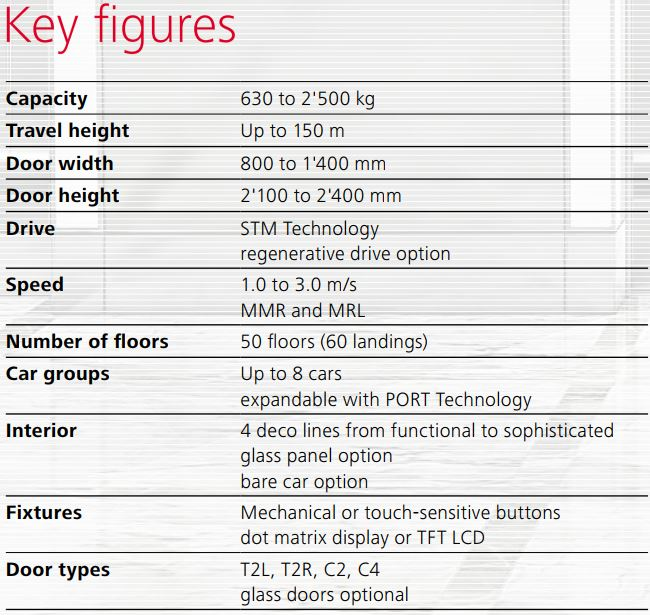
\includegraphics[clip, trim=0cm 0cm 0cm 0cm, width=0.7\textwidth]{./images/indoorclosures/elevatorfigures}
	\caption{\textit{SCHINDLER 5500} elevator key figures.}
	\label{elevatorfigures}
\end{figure}

\begin{figure}[H]
	\centering
	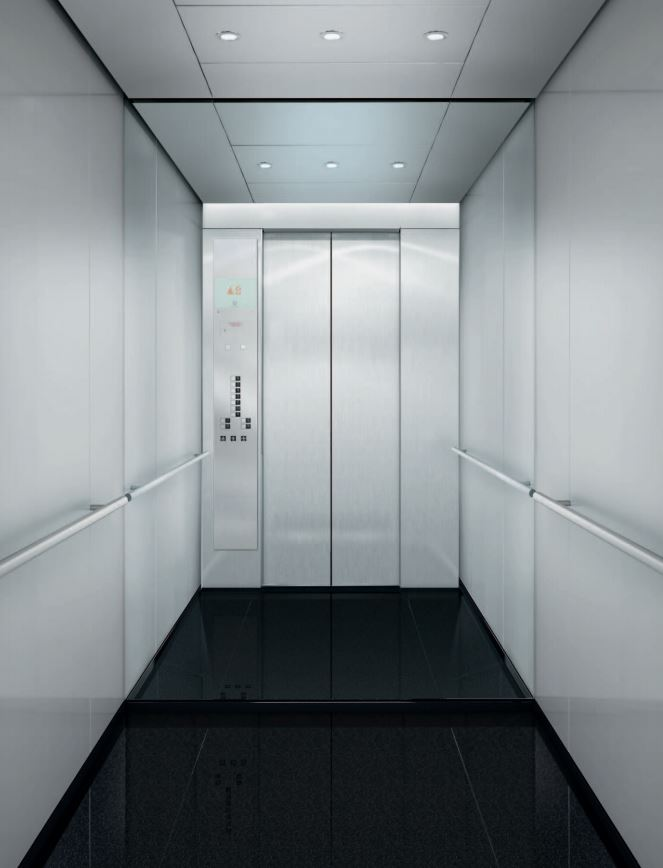
\includegraphics[clip, trim=0cm 0cm 0cm 0cm, width=0.5\textwidth]{./images/indoorclosures/elevator}
	\caption{\textit{SCHINDLER 5500} elevator used in the terminal building.}
	\label{elevator}
\end{figure}

